\documentclass[diplomskirad]{fer}
% Dodaj opciju upload za generiranje konačne verzije koja se učitava na FERWeb
% Add the option upload to generate the final version which is uploaded to FERWeb


%\usepackage{blindtext}


%--- PODACI O RADU / THESIS INFORMATION ----------------------------------------

% Naslov na engleskom jeziku / Title in English
\title{Wearable measurement system for detection and classification of speech fluency disorders}

% Naslov na hrvatskom jeziku / Title in Croatian
\naslov{Nosivi mjerni sustav za prepoznavanje i klasifikaciju poremećaja tečnosti govora}

% Broj rada / Thesis number
\brojrada{1234}

% Autor / Author
\author{Nikola Gudan}

% Mentor 
\mentor{Prof.\@ Hrvoje Džapo}

% Datum rada na engleskom jeziku / Date in English
\date{June, 2024}

% Datum rada na hrvatskom jeziku / Date in Croatian
\datum{lipanj, 2024.}

%-------------------------------------------------------------------------------


\begin{document}


% Naslovnica se automatski generira / Titlepage is automatically generated
\maketitle


%--- ZADATAK / THESIS ASSIGNMENT -----------------------------------------------

% Zadatak se ubacuje iz vanjske datoteke / Thesis assignment is included from external file
% Upiši ime PDF datoteke preuzete s FERWeb-a / Enter the filename of the PDF downloaded from FERWeb
\zadatak{Nikola Gudan - tekst zadatka - ispravljeno.pdf}


%--- ZAHVALE / ACKNOWLEDGMENT --------------------------------------------------

\begin{zahvale}
  % Ovdje upišite zahvale / Write in the acknowledgment
  TO ROKI!
\end{zahvale}


% Odovud započinje numeriranje stranica / Page numbering starts from here
\mainmatter


% Sadržaj se automatski generira / Table of contents is automatically generated
\tableofcontents


%%--- UVOD / INTRODUCTION -------------------------------------------------------
\chapter{Uvod}
\label{pog:uvod}

Placeholder
%-------------------------------------------------------------------------------
\chapter{Glavni dio}
\label{pog:glavni_dio}

\chapter{Glavna ploča}
\label{pog:mainboard}

Sustav se sastoji od dva uređaja koji rade u simbiozi. Glavna ploča služi za snimanje, obradu i pohranu glasovnih podataka i obradu i pohranu biomedicinskih parametara. Za snimanje biomedicinskih parametara koristi se narukvica. U ovom poglavlju se opisuje glavna ploča.

Zahtjevi na glavnu ploču su sljedeći:
\begin{itemize}
    \item mikrokontroler \engl{Microcontroler Unit, MCU}, dovoljno moćan za pokretanje neuralnih mreža i obradu podataka
    \item konektor za SD karticu
    \item bežična komunikacija putem Wi-Fi ili Bluetooth sučelja
    \item praćenje vremena putem RTC-a
    \item mikrofon za prikupljanje govora korisnika
    \item sučelja za testiranje i prženje koda na mikrokontroler
    \item napajanje i punjenje baterije preko USB C priključka
    \item baterijsko napajanje putem litij-ionske baterije
\end{itemize}
U daljnjem tekstu ovog poglavlja opisane su odabrane komponente, kao i razlog njihova odabira, način, razlozi i proračuni dizajna pojedinih podsustava, te dizajn, proizvodnja i testiranje PCB-a.

\section{Mikrokontroler}
Za mikrokontroler odabran je STM32F746VG baziran na Cortex-M7 arhitekturi koji integrira funkcionalnosti digitalne obrade signala, bogat sa svim potrebnim periferijama za integriranje s ostatkom sustava i dovoljno procesorske snage za obavljanje zadanog zadatka. Također, programska potpora je razvijena na razvojnom sustavu BLABLABLA, pa je ovaj mikrokontroler odabran radi lakšeg razvoja cjelokupnog sustava. Shema napajanja mikrokontrolera prikazana je na slici \ref{slk:MCU_PS}, a shema spajanja mikrokontrolera s ostatkom sustava prikazana je na slici \ref{slk:MCU_PE}.

\begin{figure}[hbt]
    \centering
    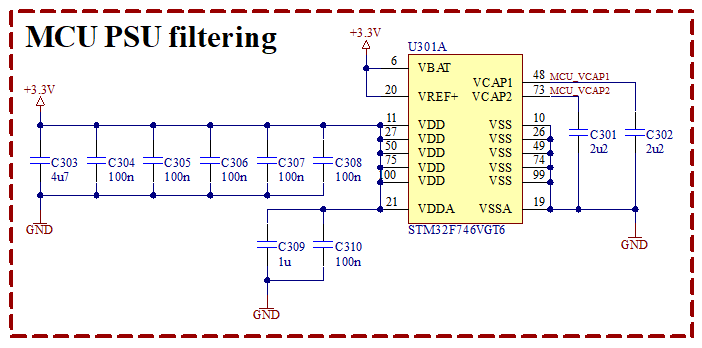
\includegraphics[width=\textwidth]{Figures/MCU_02.png}
    \caption{Shema napajanja mikrokontrolera}
    \label{slk:MCU_PS}
\end{figure}

Shema napajanja napravljena je prema uputama proizvođača \cite{stmicroelectronics:an4661}. S obzirom na to da na ovoj ploči nema analognih signala, nije potrebno raditi analogno-digitalnu pretvorbu, pa su stezaljke za napajanje analognog dijela mikrokontrolera spojene sa stezaljkama za napajanje digitalnog dijela. Također, nije potrebna precizna naponska referenca, a baterijskim napajanjem će upravljati vanjski čip, pa su te dvije stezaljke spojene na napajanje od +3.3 V.
\newpage

\begin{figure}[hbt]
    \centering
    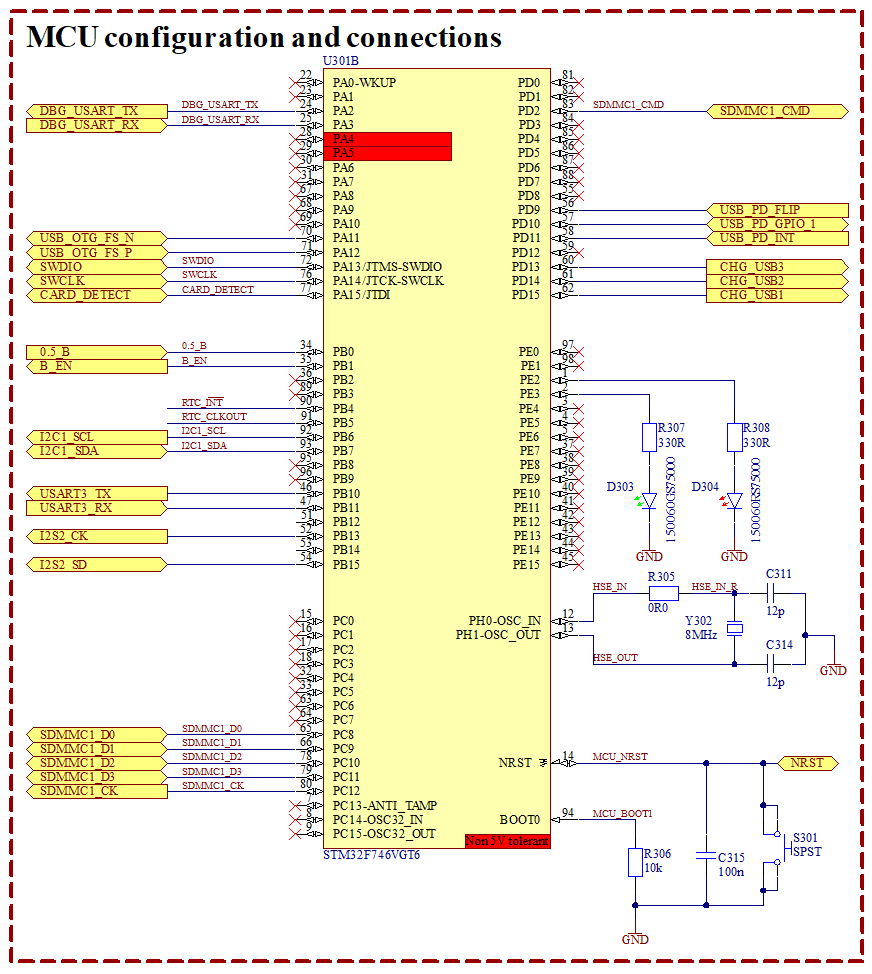
\includegraphics[width=\textwidth]{Figures/MCU_01.png}
    \caption{Shema periferije mikrokontrolera}
    \label{slk:MCU_PE}
\end{figure}

Postavljene su dvije svjetleće diode za pomoć pri programiranju i tipka za reset mikrokontrolera. Kod određivanja korištenih stezaljki za pomoć je korišteno razvojno okruženje STM32CubeIDE. Dizajn oscilatora opisan je u priručniku proizvođača STMicroelectronics \cite{stmicroelectronics:an2867}. Oscilator koji mikrokontroler koristi je Pierceov oscilator (slika \ref{slk:PIERCE}).
\begin{figure}[hbt]
    \centering
    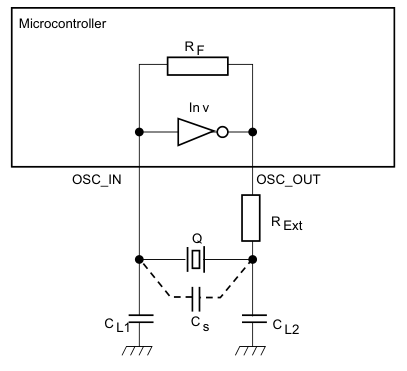
\includegraphics[width=10cm]{Figures/pierce.PNG}
    \caption{Shema Piercovog oscilatora \cite{stmicroelectronics:an2867}}
    \label{slk:PIERCE}
\end{figure}

\subsection{Pierceov oscilator}
Pierceov oscilator se sastoji od invertera \textit{Inv}, koji radi kao pojačalo, kristala \textit{Q}, otpornika u povratnoj vezi \textit{R\textsubscript{F}}, vanjskog otpornika za ograničenje izlazne struje invertera \textit{R\textsubscript{Ext}}, vanjskih kapaciteta opterećenja \textit{C\textsubscript{L1}} i \textit{C\textsubscript{L2}}, parazitskog kapaciteta PCB-a i kapaciteta između stezaljki mikrokontrolera \textit{C\textsubscript{s}}.

Uloga otpornika \textit{R\textsubscript{F}} je da natjera inverter da se ponaša poput pojačala. Otpornik povratne veze je spojen između izlaza i ulaza pojačala čime se ulaz i izlaz drže na istom naponi i prisiljava pojačalo da radi u linearnom području rada. Ovaj otpornik je integriran u mikrokontroleru zajedno s pojačalom.

Kapacitet opterećenja je ukupni kapacitet povratne veze oscilatora i mora biti jednak je kapacitetu između stezaljki kristala kako bi oscilator prooscilirao. Kapacitet opterećenja specificira proizvođač kristala i označava se s \textit{C\textsubscript{L}}. Vanjskim kondenzatorima \textit{C\textsubscript{L1}} i \textit{C\textsubscript{L2}} se postavlja kapacitet opterećenja povratne veze kako bi odgovarao kapacitetu opterećenja kristala. Kapacitet opterećenja računa se prema sljedećoj jednadžbi:
\begin{equation} \label{eq:CLOAD}
    C_L=\frac{C_{L1}\cdot C_{L2}}{C_{L1}+C_{L2}}+C_s
\end{equation}

Kod dizajna oscilatora potrebno je izračunati kritično pojačanje petlje:
\begin{equation} \label{eq:GMCRIT}
    g_{mcrit}=4\cdot ESR \cdot {(2\pi F)}^2\cdot {(C_0 + C_L)}^2
\end{equation}
gdje je \textit{F} frekvencija oscilatora, \textit{ESR} serijski otpor kristala i \textit{C\textsubscript{0}} serijski kapacitet kristala. Ovaj parametar je potrebno izračunati kako bi se moglo provjeriti hoće li se oscilator upaliti i prooscilirati. Dobiveni podatak se uspoređuje sa specificiranim vrijednostima transkonduktivnosti \textit{g\textsubscript{m}} u dokumentaciji mikrokontrolera. Da bi oscilator proradio mora se proračunati margina pojačanja i treba vrijediti:
\begin{equation} \label{eq:GMARGIN}
    {gain}_{margin}=\frac{g_m}{g_{mcrit}}>5
\end{equation}

Kako ne bi došlo do kvara kristala potrebno je ograničiti snagu koja se na njemu disipira s pomoću vanjskog otpornika \textit{R\textsubscript{Ext}}. Maksimalna snaga koja se može disipirati na kristalu naznačena je u dokumentaciji proizvođača. Ovaj otpornik s kondenzatorom \textit{C\textsubscript{L2}} formira niskopropusni filtar kako bi oscilator proradio na osnovnoj frekvenciji, a ne na višim harmonicima. Ako snaga disipirana na kristalu bude veća od maksimalne dozvoljene onda je vanjski otpornik obavezan i mora se proračunati, u suprotnom ga nije potrebno stavljati. Vrijednost otpornika se računa na sljedeći način:
\begin{equation} \label{eq:REXT}
    R_{Ext}=\frac{1}{2\pi F C_{L2}}
\end{equation}

\subsection{Dizajn oscilatora}

Oscilator je vidljiv na slici \ref{slk:MCU_PE}. Odabran je kristal NX8045GB proizvođača NDK. Njegove karakteristike su sljedeće:
\begin{itemize}
    \item \textit{C\textsubscript{L}} = 2 pF
    \item \textit{ESR} = 200 $\Omega$
    \item \textit{F} = 8 MHz
\end{itemize}
\textit{C\textsubscript{0}} nije naznačen pa se uzima vrijednost 0. Uzimajući za parazitni kapacitet \textit{C\textsubscript{s}} = 2 pF, i koristeći formulu \ref{eq:CLOAD} dobiju se vrijednosti kondenzatora \textit{C\textsubscript{L1}} = \textit{C\textsubscript{L2}} = 12 pF. Odabir parazitnog kapaciteta je odokativan jer se ne može znati unaprijed bez mjerenja dovršene tiskane pločice. Kod odabira kondenzatora potrebno je obratiti pažnju na dielektrik kondenzatora i tolerancije. Kako bi frekvencija oscilatora bila što stabilnija potrebno je koristiti temperaturno stabilan dielektrik, odnosno kondenzatore klase 1. Korišteni kondenzatori imaju C0G dielektrik. Koristeći jednadžbu \ref{eq:GMCRIT} dobiva se ${g_{mcrit} = 0.1294 \quad \textrm{mA/V}}$. Iz dokumentacije mikrokontrolera se dobiva ${g_m = 1\quad \textrm{mA/V}}$. Iz uvjeta \ref{eq:GMARGIN} dobiva se ${{gain}_{margin}=\nolinebreak 7.73}$, čime je uvjet zadovoljen. S obzirom na to da nije moguće odrediti koliko će se kristal grijati, za vanjski otpornik postavljen je otpornik vrijednosti 0 $\Omega$, pa u slučaju prevelike disipacije snage na kristalu moguće je na njegovo mjesto zalemiti otpornik odgovarajuće vrijednosti prema jednadžbi \ref{eq:REXT}.

\section{RTC}

S obzirom na to da uređaj treba uskladiti podatke s mikrofona i narukvice potrebno je precizno praćenje vremena. U tu svrhu dodan je vanjski RTC PCF8653 proizvođača NXP \cite{nxp:pcf8654}. Za ovaj čip postoji već razvijena programska podrška u ZephyrOS operacijskom sustavu za rad u stvarnom vremenu, pa je razvoj programske potpore za uređaj znatno olakšana. Shema RTC-a prikazana je na slici \ref{slk:RTC}.
\begin{figure}[hbt]
    \centering
    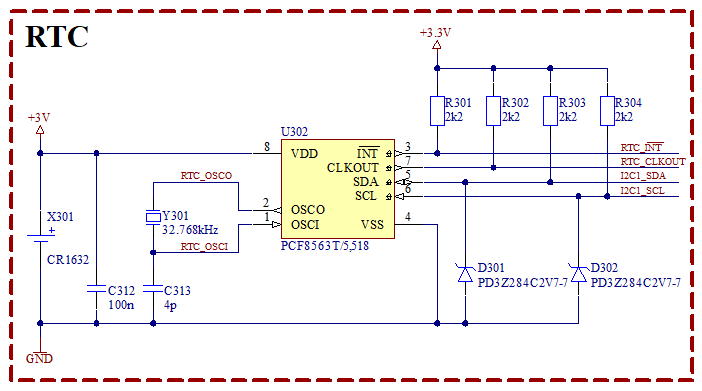
\includegraphics[width=\textwidth]{Figures/RTC.png}
    \caption{Shema RTC-a}
    \label{slk:RTC}
\end{figure}
S obzirom na to da se litij-ionska baterija, koja napaja cijeli uređaj, može isprazniti, otkopčati ili na neki drugi način se može prekinuti napajanje s vanjske baterije, RTC se napaja iz litijske baterije kako praćenje vremena ne bi bilo izgubljeno. S obzirom na to da je napon litijske baterije 3 V, a napon ostatka sustava 3.3 V, na I\textsuperscript{2}C linije dodane su Zener diode s probojnim naponom od 2.7 V, čime se maksimalni napon ograničava kako ne bi došlo do oštećenja čipa tijekom komunikacije s mikrokontrolerom.

\section{Bežična komunikacija}
\begin{figure}[hbt]
    \centering
    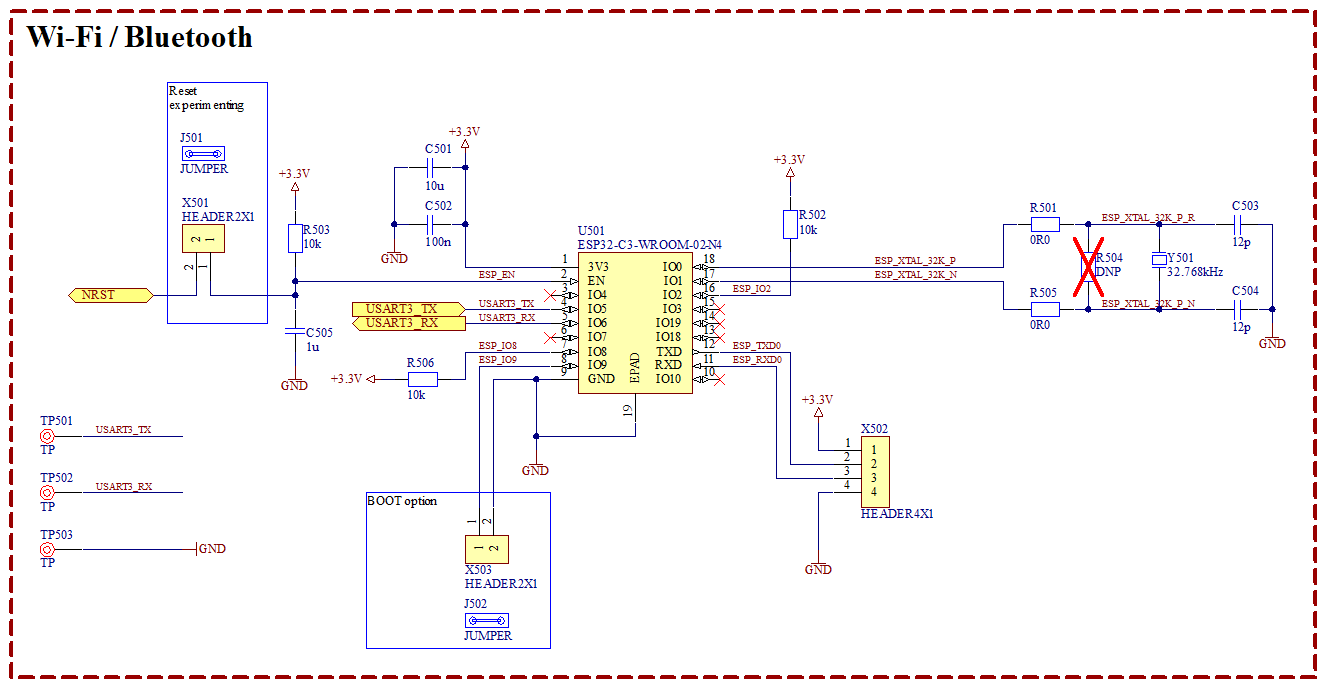
\includegraphics[width=\textwidth]{Figures/WIRELESS.png}
    \caption{Shema podsustava za bežičnu komunikaciju}
    \label{slk:WIFI}
\end{figure}
Shema podsustava za bežičnu komunikaciju prikazana je na slici \ref{slk:WIFI}. Radi lakšeg razvoja odabran je razvojni sustav ESP32-C3-WROOM-02 proizvođača Espressif Systems. Shema je razvijena prema preporukama proizvođača \cite{espressif:wroom02}. Dodan je još jedan kratkospojnik za ispitivanje funkcionalnosti reseta sustava.

\section{SD kartica i konektori}
\begin{figure}[hbt]
    \centering
    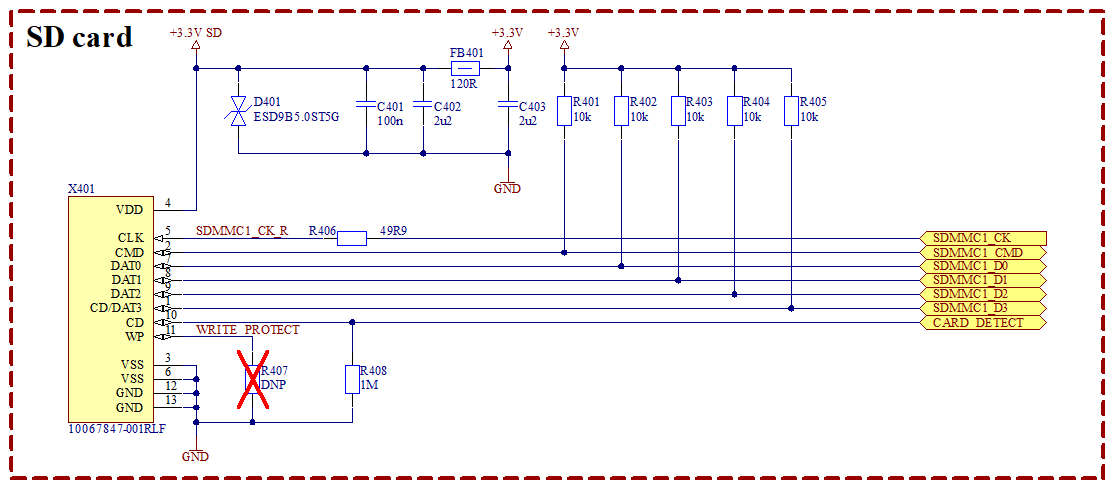
\includegraphics[width=\textwidth]{Figures/SD.png}
    \caption{Shema konektora SD kartice}
    \label{slk:SD}
\end{figure}

Za pohranu podataka na uređaju se nalazi SD kartica standardne veličine. Razlog odabira ove veličine jest taj da uređaj onda podržava i standardnu SD karticu i adapter za SD kartice manje veličine. Shema SD konektora prikazana je na slici \ref{slk:SD}. Konektor ima ESD zaštitu u obliku diode D401 i filtriranje napajanja preko mreže koja se sastoji od kondenzatora i feritne perle. Na svim komunikacijskim linijama se nalaze pritezni otpornici, a linija za takt ima terminacijski otpor od 49.9 $\Omega$ kako bi se suzbilo odzvanjanje. Kako CD stezaljka za detekciju spojene kartice ne bi ostala plutajuća dodan je pritezni otpornik od 1 M$\Omega$. Razlog odabira tako velikog otpora je unutarnji pritezni otpornik prema napajanju na SD karticama, pa se velikim otporom suzbija efekt naponskog djelila.

Za prženje korisničkog programa na mikrokontroler potreban je konektor za SWO sučelje. Dodatno, za testiranje programske podrške i komunikaciju s računalom potreban je konektor za UART sučelje. Sheme konektora prikazane su na slikama \ref{slk:UART_SWO}.
\begin{figure}[hbt]
    \centering
    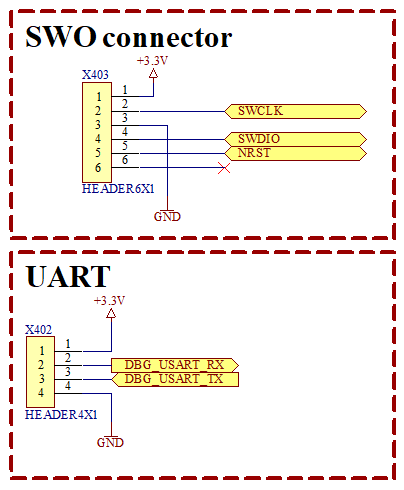
\includegraphics[width=6 cm]{Figures/SWO_UART.png}
    \caption{Shema konektora za UART i SWO sučelje}
    \label{slk:UART_SWO}
\end{figure}

Za mikrofon se koristi evaluacijska pločica STEVAL-MIC003V1 (slika \ref{slk:STEVAL}) na kojoj se nalazi MEMS mikrofon IMP34DT05 proizvođača STMicroelectronics \cite{stmicroelectronics:steval}. Za ovaj mikrofon također postoji razvijena programska podrška unutar ZephyrOS operacijskog sustava za rad u stvarnom vremenu. Ove evaluacijske pločice na sebi imaju montirane muške konektore s razmakom od 7 mm, pa se ovdje koriste ženski konektori (slika \ref{slk:MEMS}).
\begin{figure}[hbt]
    \centering
    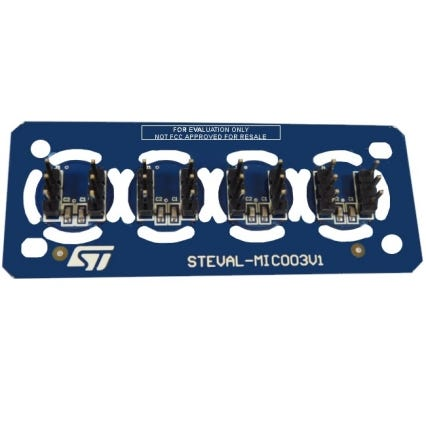
\includegraphics[width=6 cm]{Figures/STEVAL.jpg}
    \caption{STEVAL-MIC003V1}
    \label{slk:STEVAL}
\end{figure}
\begin{figure}[hbt]
    \centering
    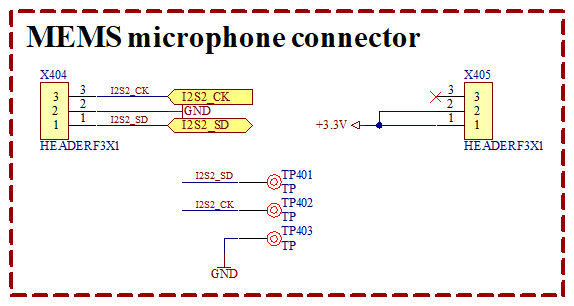
\includegraphics[width=6 cm]{Figures/MEMS.png}
    \caption{Konektori za MEMS}
    \label{slk:MEMS}
\end{figure}
Kraj konektora su postavljene testne točke za promatranje signala preko logičkog analizatora u slučaju da postoje poteškoće tijekom programiranja ili rada.

\section{Potrošnja}

Sada kada su sve komponente odabrane, moguće je napraviti proračun potrošnje kako bi se mogao dizajnirati sustav napajanja. Napravljena je tablica potrošnje za sustave koji se napajaju sa 3.3 V (tablica \ref{tab:MB3V3}). Za maksimalne i minimalne vrijednosti potrošnje uzeti su podaci iz dokumentacije komponenata, a prosječna potrošnja je uzeta odokativno jer je nemoguće znati prosječnu potrošnju bez mjerenja.
\begin{table}[htbp]
    \centering
    \caption{Potrošnja struje za sustave koji se napajaju sa 3.3 V}
    \begin{tabular}{lccc} \hline
           & Min. [mA] & Avg. [mA] & Max. [mA] \\
      MCU  & 0,00 & 60,00 & 320,00 \\
      RTC  & 0,00 & 0,80 & 50,00 \\
      SD Card & 1,25 & 25,00 & 100,00 \\
      MEMS & 0,00 & 0,65 & 10,00 \\
      Wireless & 13,00 & 82,00 & 350,00 \\ \hline
      Total on SYS & 14,25 & 168,45 & 830,00 \\ \hline
    \end{tabular}%
    \label{tab:MB3V3}%
\end{table}%
Sada je moguće odabrati prikladne komponente za napajanje.

\section{Napajanje i punjač baterije}
Za punjač baterije odabran je BQ24166 proizvođača Texas Instruments (slika \ref{slk:BQ24166}). Ovaj integrirani krug u sebi ima integriran sustav za upravljanje tokom snage \cite{ti:bq24166}. BQ24166 se može napajati s dva ulaza; ulaz za USB ili ulaz za druge vrste napajanja (AC/DC adapter, DC laboratorijski izvor napajanja, itd.), a da pritom u isto vrijeme puni bateriju i na svom izlazu daje napon baterije, s tim da izlazni napon neće pasti ispod 3.5 V. U tu svrhu u čip je ugrađen silazni prekidački regulator napona, kako bi se kod punjenja baterije konstantnim naponom dobio izlazni napon od 4.2 V potreban za punjenje. Ako na ulaz čipa nije spojeno ništa, onda se na izlaz direktno prosljeđuje napon baterije. U slučaju da napon baterije padne ispod 3.5 V, a da pritom ništa nije spojeno na ulaz čipa, izlazni napon se regulira na 3.5 V, čime se baterija može u potpunosti iskoristiti. Ovaj čip također ima ugrađene zaštite od prednapona, a jednim otpornikom moguće je i programirati prekostrujnu zaštitu. Također je jednim otpornikom moguće i programirati maksimalnu struju punjenja baterije.
\begin{figure}[hbt]
    \centering
    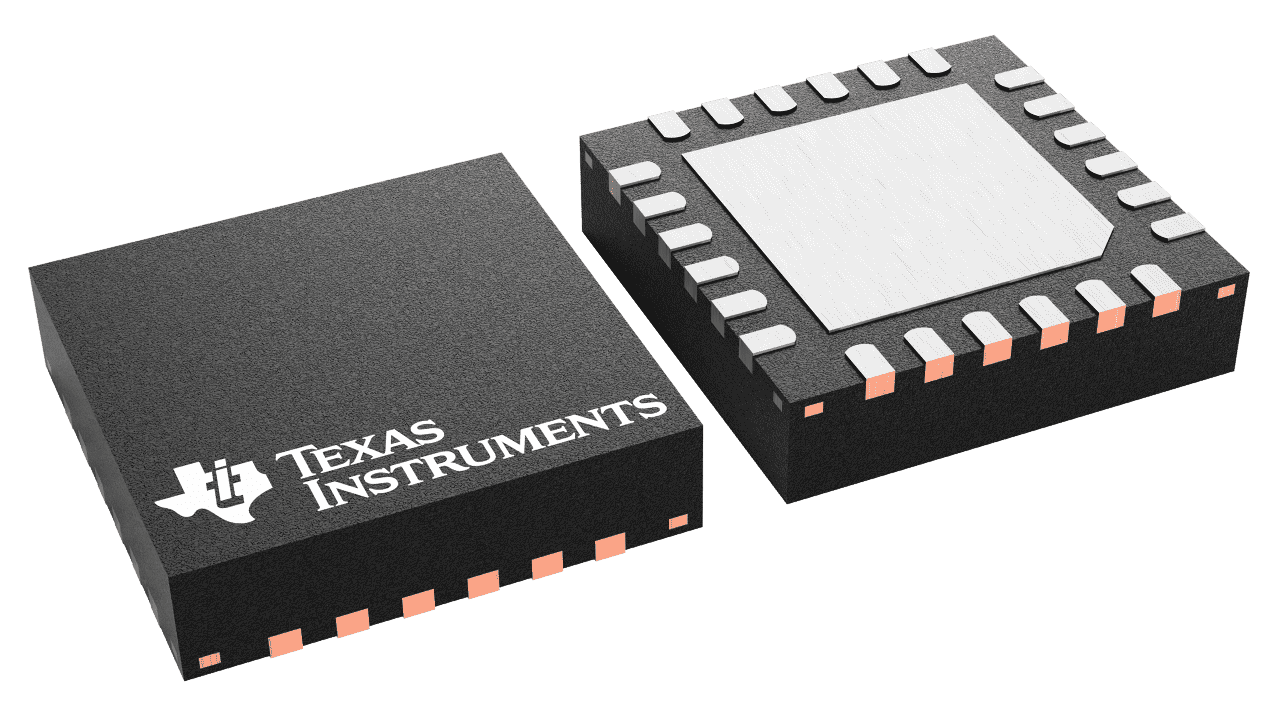
\includegraphics[width = 10 cm]{Figures/bq24166.png}
    \caption{BQ24166 u QFN kućištu}
    \label{slk:BQ24166}
\end{figure}
Shema baterijskog punjača prikazana je na slici \ref{slk:MB_BATCHG}. Blokadni kondenzatori su postavljeni prema uputama proizvođača, a potrebno je bilo odabrati odgovarajuće otpornike za programiranje prekostrujne zaštite i maksimalne struje punjenja, kao i prikladnu zavojnicu. Kako bi se navedene komponente odabrale na odgovarajuć način, potrebno je znati izlaznu struju iz punjača.
\begin{figure}[hbt]
    \centering
    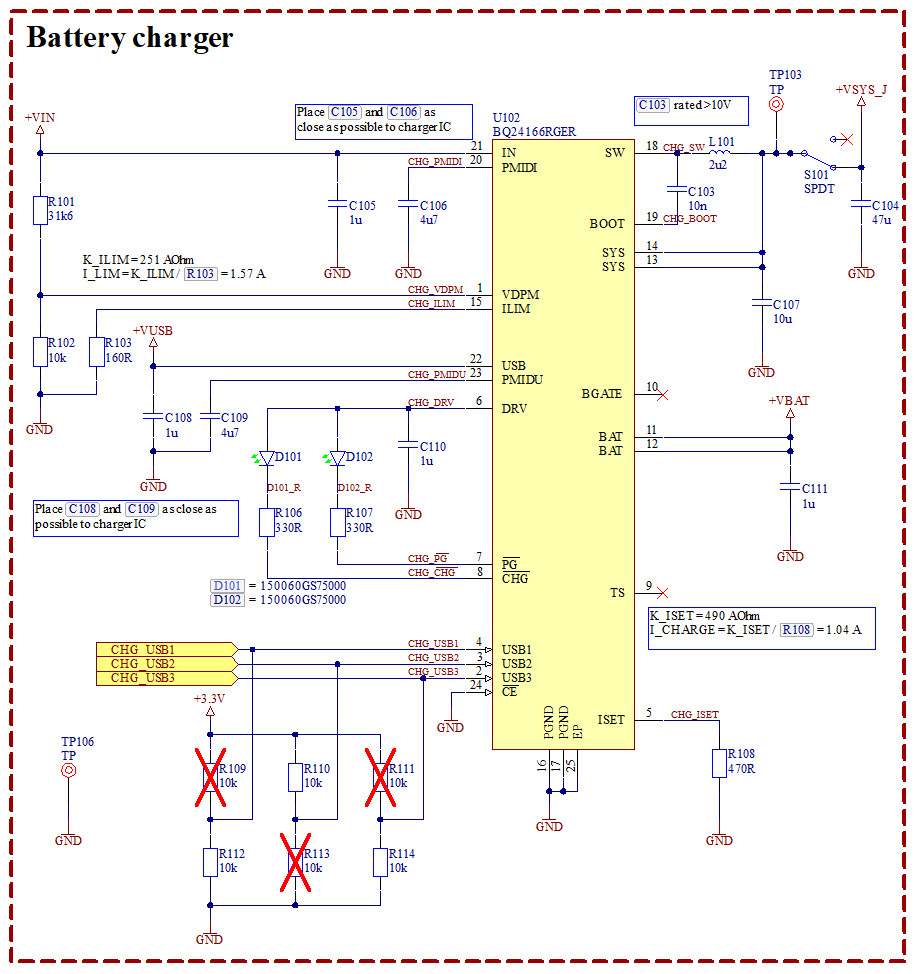
\includegraphics[width = \textwidth]{Figures/MB_BATCHG.png}
    \caption{Shema baterijskog punjača}
    \label{slk:MB_BATCHG}
\end{figure}

Na izlazu punjača se nalazi linearni regulator napona s niskim padom napona (190 mV na struji od 1.5 A) koji regulira napon na 3.3 V (slika \ref{slk:MB_LDO}). Imajući na umu da je ulazna struja linearnog regulatora otprilike ista kao i izlazna struja, dobiva se izlazna struja baterijskog punjača, što odgavara proračunu iz tablice \ref{tab:MB3V3}, a to je ujedno i struja koju daje baterija. Da bi se dobila maksimalna ulazna struja punjača potrebno je uzeti u obzir najgori mogući slučaj: baterija je odspojena, potrošnja sustava je maksimalna. Unutar punjača se nalazi silazni pretvarač, dakle vrijedi:
\begin{equation}
    P_{IZ}=\eta \cdot P_{UL}
\end{equation}
\begin{equation} \label{eq:BUCK}
    U_{IZ}\cdot I_{IZ}=\eta \cdot U_{UL} \cdot I_{UL}
\end{equation}
gdje je \textit{U\textsubscript{IZ}} i \textit{I\textsubscript{IZ}} izlazni napon, odnosno struja, \textit{U\textsubscript{UL}} i \textit{I\textsubscript{UL}}, ulazni napon, odnosno struja, a $\eta$ učinkovitost. Bacajući pogled u dokumentaciju proizvođača, može se uzeti efikasnost od 90 \% (slika \ref{slk:EFFICIENCY}).
\begin{figure}[hbt]
    \centering
    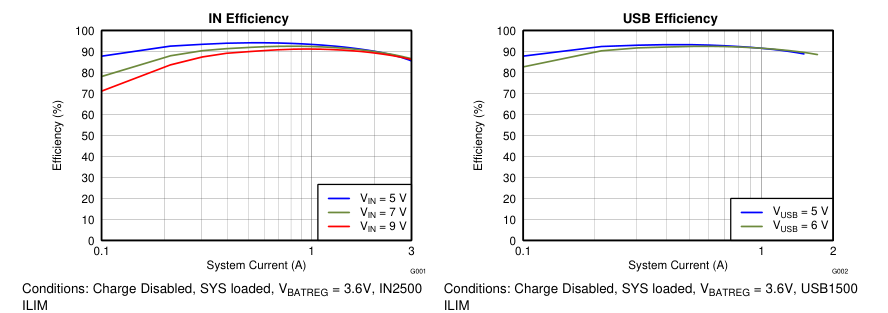
\includegraphics[width=\textwidth]{Figures/EFFICIENCY.PNG}
    \caption{Ovisnost efikasnosti o izlaznoj struji punjača \cite{ti:bq24166}}
    \label{slk:EFFICIENCY}
\end{figure}
Iz jednadžbe \ref{eq:BUCK} se sada može dobiti izraz za ulaznu struju:
\begin{equation} \label{eq:IN_CURR}
    I_{UL}=\frac{\eta \cdot U_{IZ} \cdot I_{IZ}}{U_{UL}}
\end{equation}
Iz jednadžbe \ref{eq:IN_CURR} je vidljivo da će ulazna struja biti najveća kada je ulazni napon što manji, što u ovom slučaju iznosi 5 V. Za izlazni napon se također uzima najgori slučaj od 4.2 V. Sada se za maksimalnu ulaznu struju punjača uz odspojenu bateriju dobiva iznos od ${I_{UL,BATOFF} = 627.48\quad \textrm{mA}}$.
\begin{figure}[hbt]
    \centering
    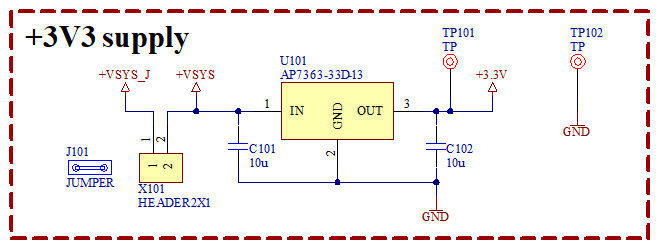
\includegraphics[width = 10 cm]{Figures/MB_LDO.png}
    \caption{Linearni regulator napona}
    \label{slk:MB_LDO}
\end{figure}

Imajući na umu da će do maksimalne potrošnje doći rijetko kada, ako uopće, i činjenicu da će sustav imati mogućnost ulaska u način rada mirovanja, može se uzeti kapacitet baterije od 2 Ah, čime se postiže balans trajanja baterije i cijene. U tom slučaju dovoljno je ograničiti punjenje baterije na 1 A, a izračun otpornika je vidljiv na shemi (slika \ref{slk:MB_BATCHG}). Odgovarajuće konstante za izračun otpornika su dobivene iz dokumentacije proizvođača. Sada je isto pomoću jednadžbe \ref{eq:IN_CURR} moguće izračunati ulazni struju; ${I_{UL,BATCHG} = 756\quad \textrm{mA}}$. Ukupna maksimalna ulazna struja je stoga:
\begin{equation}
    I_{UL,MAX}=I_{UL,BATCHG}+I_{UL,BATOFF} = 1.38 A
\end{equation}
Dodajući malo sigurnosne margine, za prekostrujnu zaštitu se onda uzima 1.5 A. Za potrebe testiranja i otklanjanje evenutalnih grešaka na ulaz linearnog regulatora dodan je kratkospojnik.

S obzirom na mnoge opasnosti koje litij-ionske baterije nude, potrebno je dizajnirati prikladnu zaštitu za bateriju. U tu svrhu odabran je BQ29700 proizvođača Texas Instruments,

Nešto


%-------------------------------------------------------------------------------
\chapter{Rezultati i rasprava}
\label{pog:rezultati_i_rasprava}

Nešto


%--- ZAKLJUČAK / CONCLUSION ----------------------------------------------------
\chapter{Zaključak}
\label{pog:zakljucak}


%--- LITERATURA / REFERENCES ---------------------------------------------------

% Literatura se automatski generira iz zadane .bib datoteke / References are automatically generated from the supplied .bib file
% Upiši ime BibTeX datoteke bez .bib nastavka / Enter the name of the BibTeX file without .bib extension
\bibliography{literatura}



%--- SAŽETAK / ABSTRACT --------------------------------------------------------

% Sažetak na hrvatskom
\begin{sazetak}
Projektiranje i izrada sklopovlja za nosivi mjerni sustav za prepoznavanje i klasifikaciju poremećaja tečnosti govora. Sustav se sastoji od dva nosiva uređaja. Jedan je za snimanje glasovnih podataka s MEMS mikrofonom, obradu podataka i njihovu pohranu na SD karticu. Drugi je za snimanje biomedicinskih signala (PPG i EDR) u obliku nosive narukvice. Oba sustava imaju funkcije bežične komunikacije preko Wi-Fi ili Bluetooth sučelja, napajanje s litij-ionskom baterijom te napajanje i punjenje preko USB C sučelja. Opisani su dizajn sustava, projektiranje tiskane pločice i funkcionalno ispitivanje sastavljenih uređaja.
\end{sazetak}

\begin{kljucnerijeci}
MEMS mikrofon, SD kartica, PPG, EDR, Wi-Fi, Bluetooth, litij-ionska baterija, USB C sučelje
\end{kljucnerijeci}


% Abstract in English
\begin{abstract}
  Enter the abstract in English.
\end{abstract}

\begin{keywords}
  the first keyword; the second keyword; the third keyword
\end{keywords}


%--- PRIVITCI / APPENDIX -------------------------------------------------------

% Sva poglavlja koja slijede će biti označena slovom i riječi privitak / All following chapters will be denoted with an appendix and a letter
\backmatter

\chapter{The Code}


\end{document}
